\section{Localization System}
The basic idea behind our localization system implementation is to capture a frame at real time by a camera, then detect and decode the QR code in it. After that, we will be able to restore the QR code's global position from the server using the decoded data, \color{blue}which is described at...(write where) \color{black}. Now, we only need to calculate the camera's position relative to the QR code, and then add the result together with the QR code's global position as follows:
\[ user\_global\_position = QR\_global\_position +  camera\_relative\_position\]
As we just mentioned, the QR code's global position is stored at a server so there is nothing to calculate here, but this is not the case of the camera's relative position. The process of calculating the later is somewhat complicated and not short, and there are several things that need to be calculated first, such as the QR code corners locations at the image frame, camera matrix, and the camera distortion coefficients. There are libraries for calculating these values, such as OpenCV, g2o, libmv, and Kalibr. We are going to use OpenCV since it very simple and can be used with kotlin easily.

Everything related to the localization will be running at a separate thread from the main thread. This enables the System to perform other tasks simultaneously and independently.

\subsection{Camera Calibration}
Camera Calibration is the process of calculating the camera's parameters in order to figure out how exactly does the camera transform a 3D scene into a 2D image. In our localization implementation, calibration is crucial since we need to estimate the camera's position relative to the detected QR code. 

We mentioned \color{blue}at...(write where) \color{black} that users can chose the camera they want to use from the settings after connecting it to the phone. This approach rise the need of calibration system that users can use since the cameras' parameters are distinct and not known. The basic idea behind our camera calibration implementation is to take multiple photos by the camera to a known pattern, then try to accurately locate some points at these photos. Then compare these estimated points to their physical locations of points in the calibration pattern (usually on a flat surface) in the real-world coordinate system. By comparing the 2D points in the images to their known 3D locations in the real-world coordinate system, we will be able to calculate accurate values of the camera intrinsic values and distortion coefficients.

\begin{figure}[h] % [h] forces the figure to be placed exactly here in the text
	\centering
	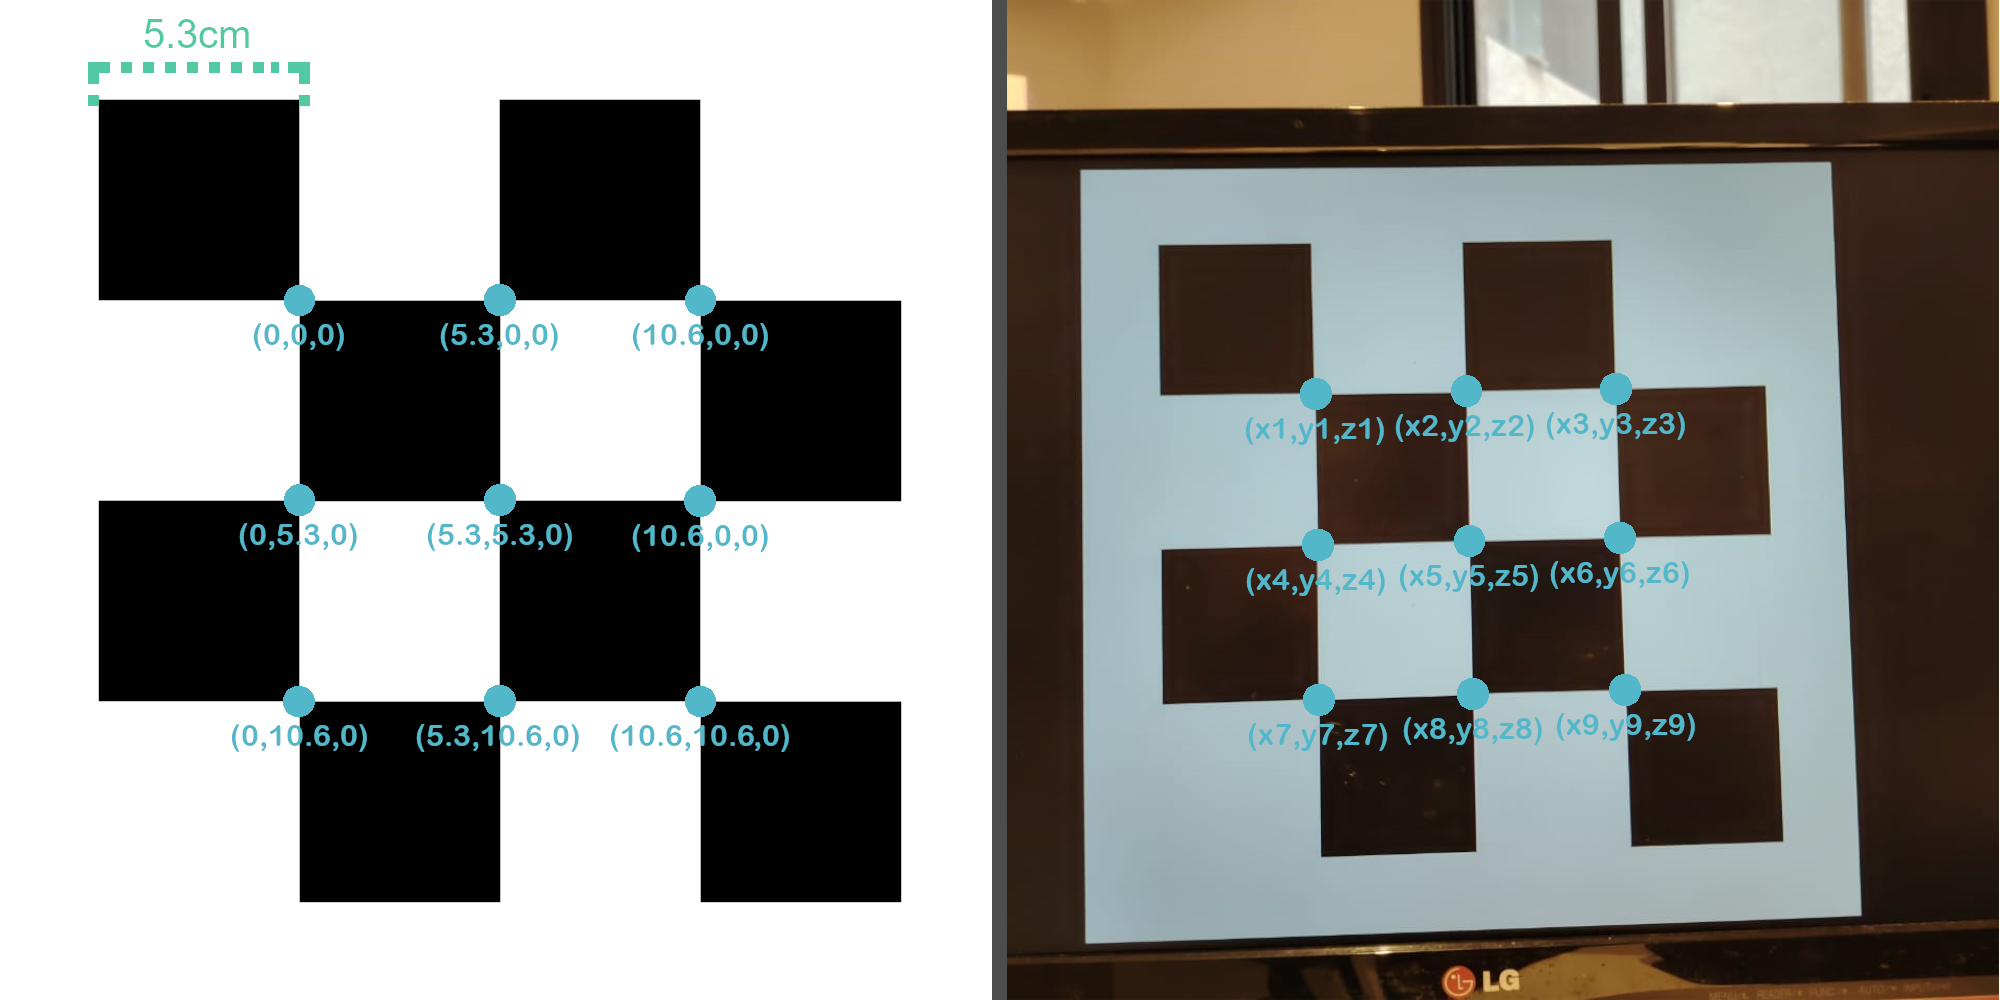
\includegraphics[width=\textwidth]{assets/ch3/calibration illustration image/calibration illustration image.png}
	\caption{ The left image represents the calibration pattern's real world inner points locations. While on the other hand, the right image shows the estimated inner  points locations. }
	\label{Calibration_Illustrator}
\end{figure}

Each camera need to be calibrated at least once at the first time. Then the camera parameters will be stored at the phone storage for reusing in the future. At first, users need to specify the number of rows and columns at the pattern and the width/height of each square in real world units. Then they need to take multiple photos to the pattern at different angles and distances and start the calibration process. After this point, everything else will be done automatically without the need of the users actions no more. 

Now let us dive into the implementations details. At first the program will iterate through each photo trying to estimate their inner corners points locations using the following OpenCV function:
\begin{lstlisting}[language=Java]
boolean findChessboardCorners(
	Mat image,
	Size patternSize,
	MatOfPoint2f corners
)
\end{lstlisting}

\subparagraph{Params:}

\begin{itemize}
	\item \textbf{image:}
	The current photo of the pattern.
	\item \textbf{patternSize:}
	Number of inner corners per a chessboard row and column.
	\item \textbf{corners:}
	Output array of detected corners.
\end{itemize}

After that, we used the OpenCV function cornerSubPix to refine the detected points. Finally, we used the following OpenCV function for pose estimation:
\begin{lstlisting}[language=Java]
double calibrateCamera(
	List<Mat> objectPoints,
	List<Mat> imagePoints, 
	Size imageSize, 
	Mat cameraMatrix, 
	Mat distCoeffs, 
	List<Mat> rvecs, 
	List<Mat> tvecs
)
\end{lstlisting}

\subparagraph{Params:}

\begin{itemize}
	\item \textbf{objectPoints:}
	List of real world inner points locations for each image.
	\item \textbf{imagePoints:}
	List of estimated inner points locations for each image.
	\item \textbf{imageSize:}
	Size of the calibrated pattern photo.
	\item \textbf{cameraMatrix:}
	Output matrix for the camera intrinsic values.
	\item \textbf{distCoeffs:}
	Output matrix for the camera distortion coefficients.
	\item \textbf{rvecs:}
	Output list contains the rotation of the calibration patterns for each image.
	\item \textbf{tvecs:}
	Output list contains the translation of the calibration patterns for each image.
\end{itemize}

\subsection{Camera's Relative Position}
The first step is to capture frames using a camera at real time. There are several libraries for doing so in Android devices, such as Camera2, and CameraX. It is recommended for most developers to use CameraX library, since it supports the vast majority of Android devices, and provides a simple and easy to use API - unlike Camera2 - that spares users from dealing with compatibility issues and other low level details. See \cite{whichCameraLibToUse} for more info.

Each captured frame will be passed to a function for QR code detecting, decoding, and pose estimation, so finally we can calculate camera's relative position. For QR code detecting, there are bunch of useful libraries we can for QR code detecting and decoding as we mentioned previously in the background section. We choose Google's ML kit due to its simplicity and good performance. After successfully detecting the QR code, Google's ML kit will calculate the QR code corners locations for us.

Finally, we use OpenCV's solvePnP to calculate the QR pose function as follow:

\begin{lstlisting}[language=Java]
boolean solvePnP(
	MatOfPoint3f objectPoints, 
	MatOfPoint2f imagePoints, 
	Mat cameraMatrix, 
	MatOfDouble distCoeffs, 
	Mat rvec, 
	Mat tvec
)
\end{lstlisting}

\subparagraph{Params:}

\begin{itemize}
	\item \textbf{objectPoints:}
	The QR code's four corners locations relative to its center in real world units, such as cm, mm, etc.
	\item \textbf{imagePoints:}
	The locations of the QR code's corners inside the captured frame in pixels.
	
	\item \textbf{cameraMatrix \& distCoeffs:}
	These two are crucial for calculating the QR code's pose since they represent the intrinsic values of a camera and its distortion coefficients.
	
	\item \textbf{rvec \& tvec:}
	These are output vectors for the code's rotation(rvec) and translation(tvec) relative to the camera.
\end{itemize}

Now we got the QR code's translation vector relative to the camera, we just multiply it with -1 to get the camera translation relative to the QR code.